\documentclass[a4paper,12pt]{article}

%%% Работа с русским языком
\usepackage{cmap}					% поиск в PDF
\usepackage{mathtext} 				% русские буквы в формулах
\usepackage[T2A]{fontenc}			% кодировка
\usepackage[utf8]{inputenc}			% кодировка исходного текста
\usepackage[english,russian]{babel}	% локализация и переносы
\usepackage{xcolor}
\usepackage{hyperref}
 % Цвета для гиперссылок
\definecolor{linkcolor}{HTML}{799B03} % цвет ссылок
\definecolor{urlcolor}{HTML}{799B03} % цвет гиперссылок

\hypersetup{pdfstartview=FitH,  linkcolor=linkcolor,urlcolor=urlcolor, colorlinks=true}

%%% Дополнительная работа с математикой
\usepackage{amsfonts,amssymb,amsthm,mathtools} % AMS
\usepackage{amsmath}
\usepackage{icomma} % "Умная" запятая: $0,2$ --- число, $0, 2$ --- перечисление

%% Номера формул
%\mathtoolsset{showonlyrefs=true} % Показывать номера только у тех формул, на которые есть \eqref{} в тексте.

%% Шрифты
\usepackage{euscript}	 % Шрифт Евклид
\usepackage{mathrsfs} % Красивый матшрифт

%% Свои команды
\DeclareMathOperator{\sgn}{\mathop{sgn}}

\newcommand*{\hm}[1]{#1\nobreak\discretionary{}
{\hbox{$\mathsurround=0pt #1$}}{}}
% графика
\usepackage{graphicx}
\graphicspath{{pictures/}}
\DeclareGraphicsExtensions{.pdf,.png,.jpg}
\author{Бурмашев Григорий}
\title{Матан, коллок - 1 }
\date{\today}
\begin{document}
\begin{center}
Бурмашев Григорий. 208. Дискра-6
\end{center}
\section*{Номер 1}
Можно заметить, что вершины связаны, если они отличаются друг от друга на 3 или на 5. Тогда мы можем построить цикл вида (или любой другой подобный):
\begin{center}
8 5 0 3 6 9 5 8 3 0 5 2 7 4 1 6 9 4 7 2 5 8 $ \circlearrowleft $
\end{center}
$\rightarrow$ весь граф является сильно связным и у нас 1 компонентна сильной связности
\begin{center}
\textbf{Ответ:} 1 компонентна сильной связности
\end{center}
\section*{Номер 2}
Построим неориентированный граф следующим образом:

Пусть у нас есть вершина A. Соединим её с вершинами B, С и D. При этом эти вершины между собой напрямую не связаны. Тогда у нас есть следующий путь, который проходит через каждое ребро ровно 2 раза:
\[
A - D - A - C - A - B - A
\]
При этом в этом графе нет эйлерового цикла, т.к в нем есть вершина нечетной степени (A), что противоречит условию существования эйлерового цикла в неориентированном графе.

Изображение:
\begin{center}
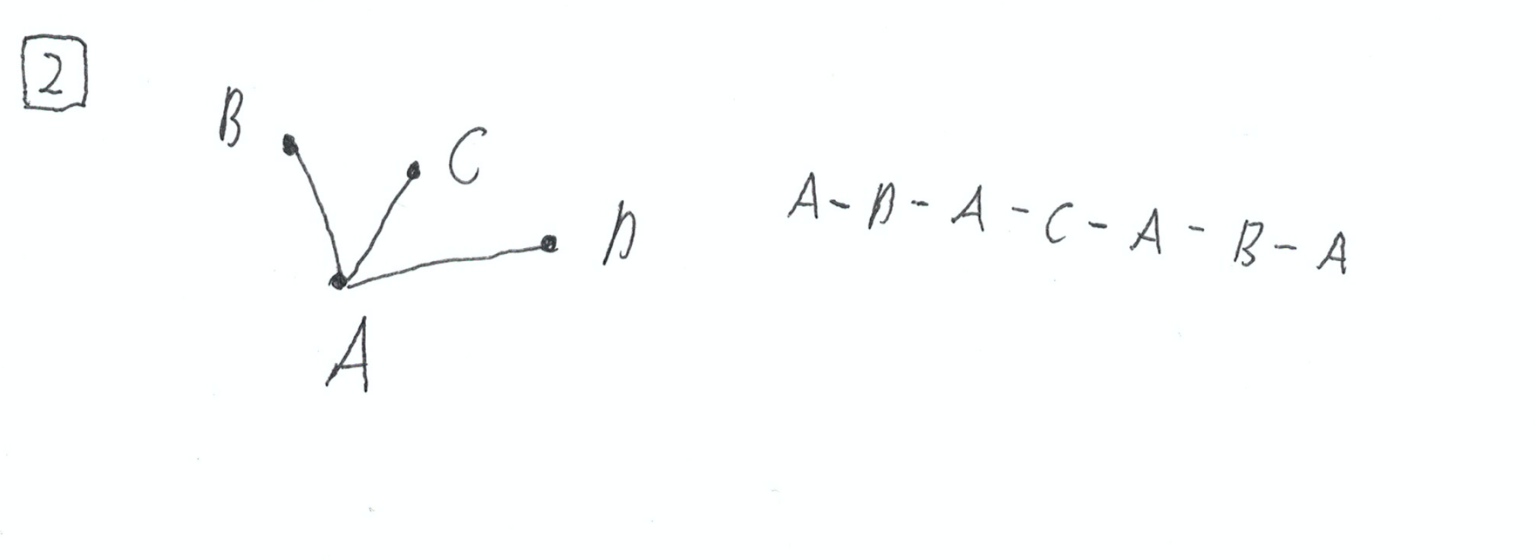
\includegraphics[scale=0.4]{2.png}
\end{center}
\begin{center}
\textbf{Ответ:} нет 
\end{center}
\section*{Номер 3}
Построим граф на трех вершинах A, B и C, в котором из любой вершины в любую другую ведет ровно один простой путь. Но мы видим, что у вершины B, которая является исходящей для A и C, степень вершины равняется 2.

Изображение:
\begin{center}
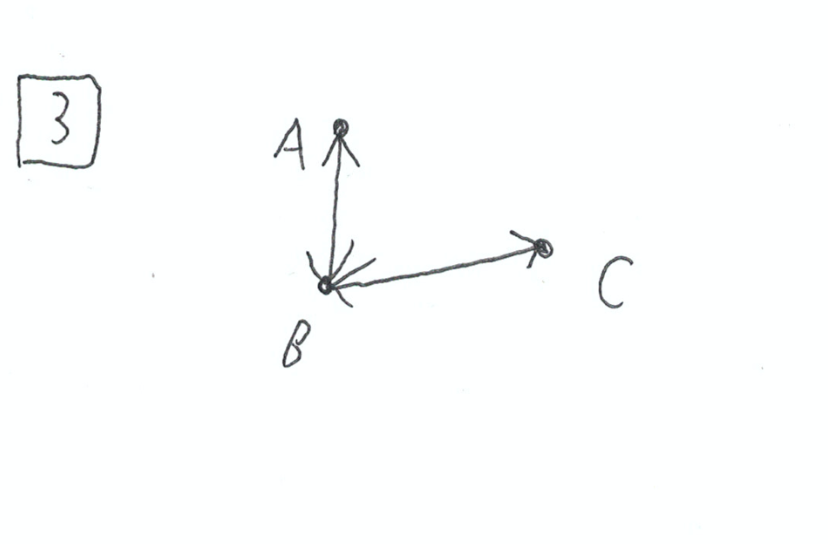
\includegraphics[scale=0.4]{3.png}
\end{center}
\begin{center}
\textbf{Ответ:} нет
\end{center}
\section*{Номер 4}
\subsection*{а) }
Всего у нас 64 строки, в каждую из которых у нас может поместиться 1 слово длины 6. Двоичных слов длины 6 у нас $2^6 = 64$. Т.к на каждой из 6 позиций числа может стоять 2 варианта (0 и 1). $\rightarrow$ мы можем поместить все 64 слова в 64 строки.
\begin{center}
\textbf{Ответ:} да
\end{center} 
\subsection*{б)}
Из пункта а) следует, что таблица состоит из различных двоичных слов длины 6. 

Построим таблицу следующим образом:
\begin{center}
\begin{tabular}{|c|c|c|c|c|c|}
\hline
 0& 0 & 0 &  0&  0& 0 \\
\hline
 0&0  & 0 & 0 &  0& 1 \\
\hline
 0&  0&0  & 0 &1 &  0\\
\hline
$\ldots $ & $ \ldots $& $\ldots $ & $ \ldots$&$\ldots$  & $\ldots$ \\
\hline
 1& 1 & 1 &  1&  1& 1 \\
\hline
\end{tabular}
\end{center}

Т.е расставим сверху вниз все двоичные числа длины 6 в порядке их возрастания. Зафиксируем случайную строку. При удалении любой единицы из любой вышестоящей строки мы уменьшим двоичное число, а следовательно поднимем его еще выше в таблице (т.к числа расставлены в порядке возрастания) $\rightarrow$ получить число из фиксированной строки невозможно и условие пункта б) выполняется
\begin{center}
\textbf{Ответ:} да
\end{center}
\section*{в)}
Рассмотрим случай, когда числа стоят \textbf{не} в порядке возрастания. Тогда для для какой-то как минимум одной строки мы сможем найти вышестоящую строчку, где будут стоять единицы на тех же позициях. В ней можно будет заменить все другие единицы на нули и получить число из нижней строки. Тогда условие пункта б) нарушается и значит числа таки стоят в порядке возрастания. В таком случае, на 57й позиции стоит число  $11100 \neq 011100$
\begin{center}
\textbf{Ответ:} нет
\end{center}
\section*{Номер 6}
Воспользуемся методом математической индукции:
\begin{itemize}
\item База: при n = 2 :

Очевидно,что есть простой путь, включающий в себя обе вершины
\begin{center}
\textbf{Верно}
\end{center}
\item Переход: пусть верно для n, т.е $\exists$ граф на n вершинах, содержащий в себе простой путь через все вершины. Докажем, что это верно для $n+1$:
\end{itemize}
Мы добавляем в граф $n+1$ вершину A. Пусть первая точка в простом графе на $n$ вершинах есть $V_1$, а последняя точка в простом пути на n вершинах -- $V_n$ Рассмотрим все возможные варианты:
\begin{enumerate}
\item Если существует ребро из вершины A в вершину $V_1$, то мы просто начинаем путь из вершины A и опять получаем простой путь, проходящий через все вершины
\begin{center}
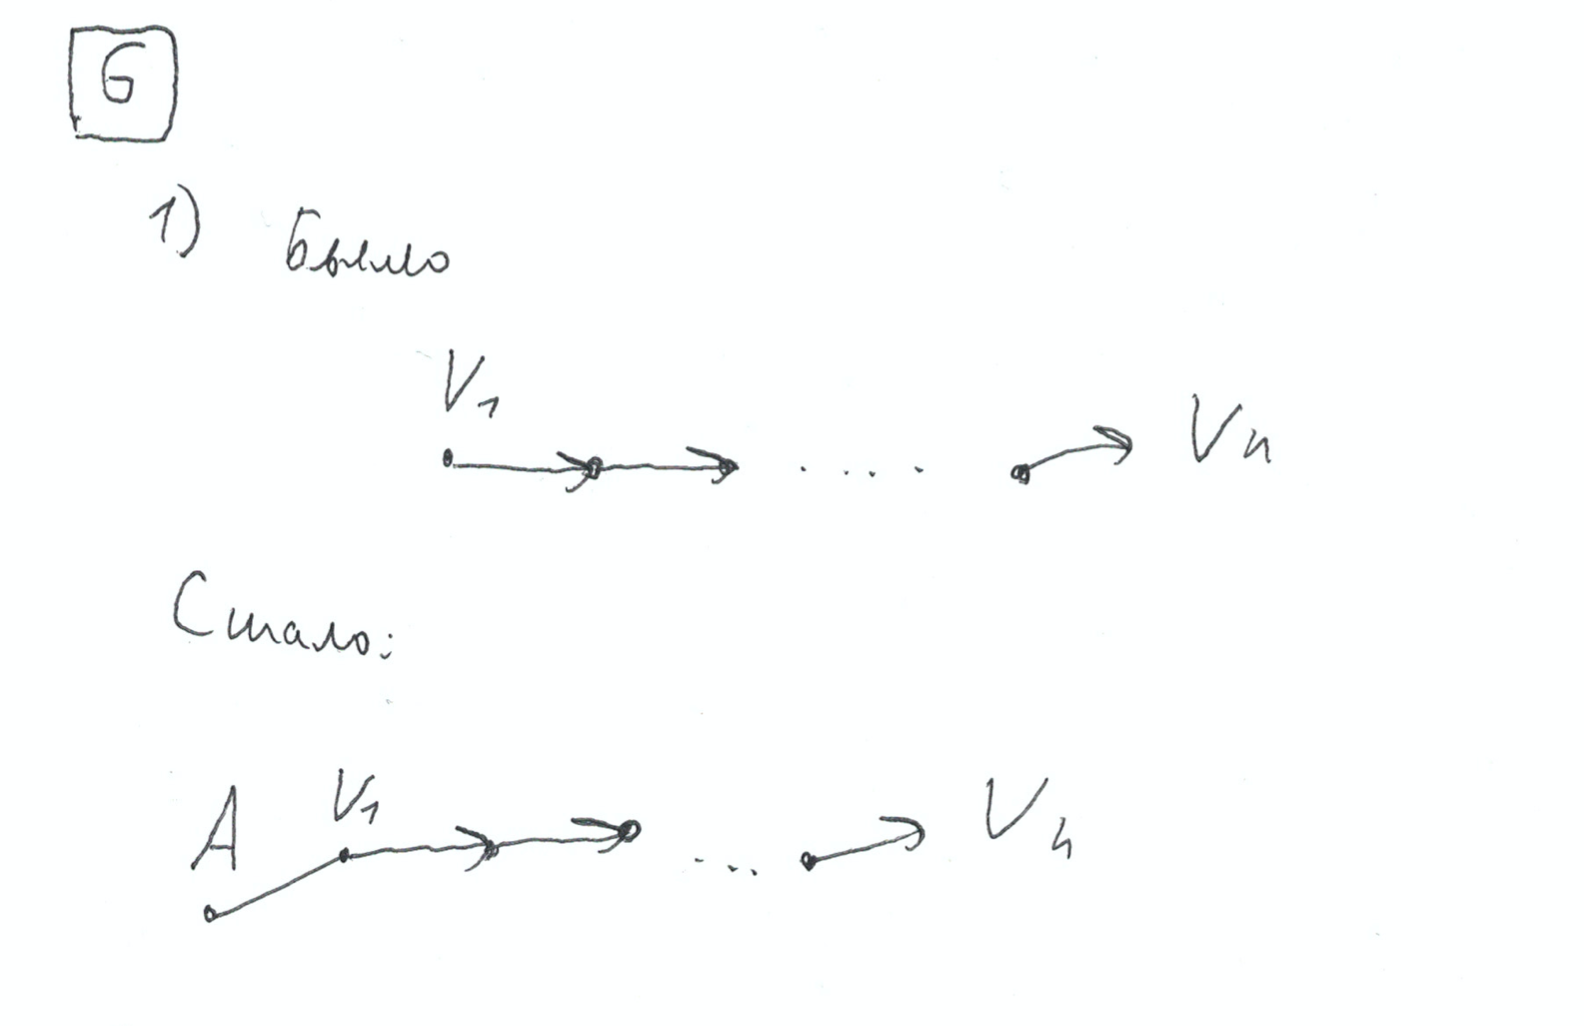
\includegraphics[scale=0.35]{6.1.png}
\end{center}
\item Если существует ребро из $V_n$ в  вершину A, то мы просто заканчиваем путь в вершине A и он опять является простым путем, проходящим через все вершины.
\begin{center}
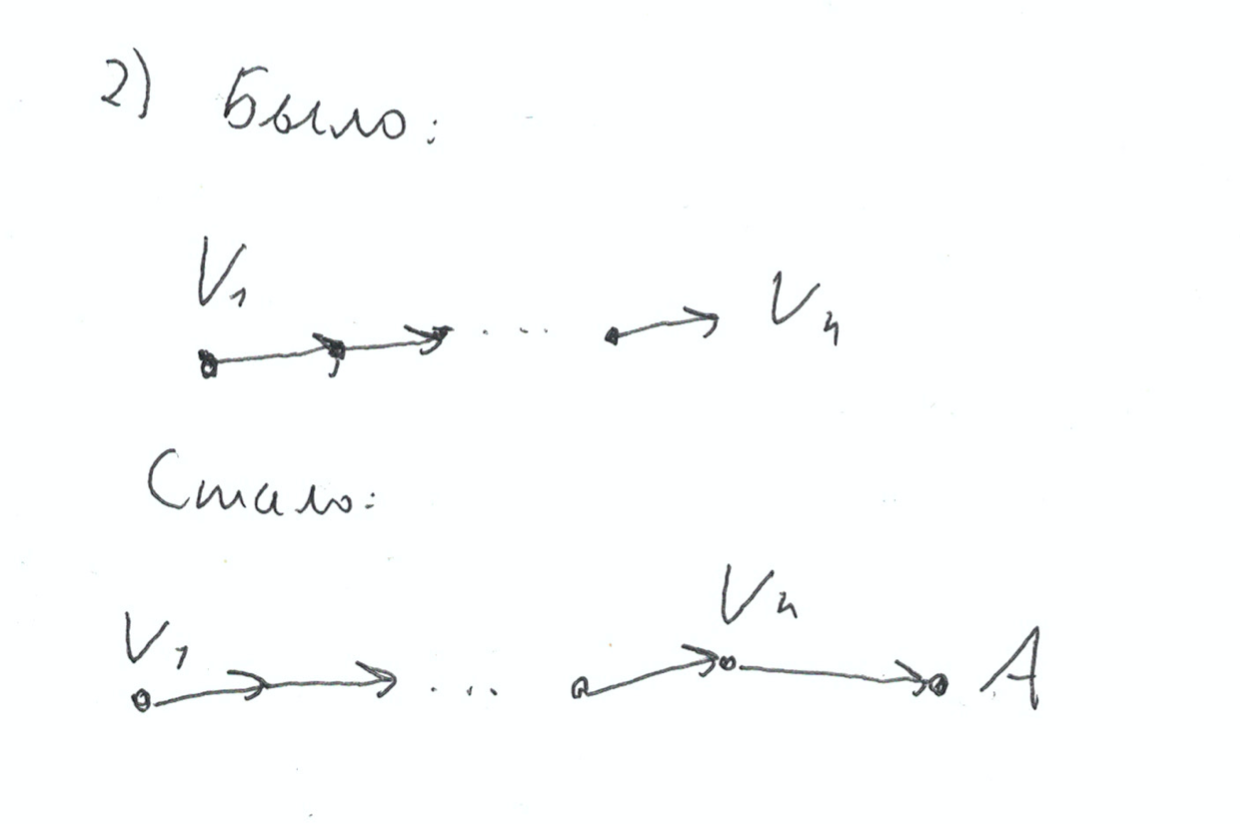
\includegraphics[scale=0.4]{6.2.png}
\end{center}
\newpage
\item Если вершина A находится в графе где-то между $V_1$ и $V_n$, т.е есть путь из $V_1$ в A и из A в $V_n$, то найдется такая $V_k$, что из нее будет ребро в A, а из A ребро в следующую вершину в простом цикле на n вершинах $\rightarrow$ мы опять получаем простой путь, проходящий через все вершины.
\begin{center}
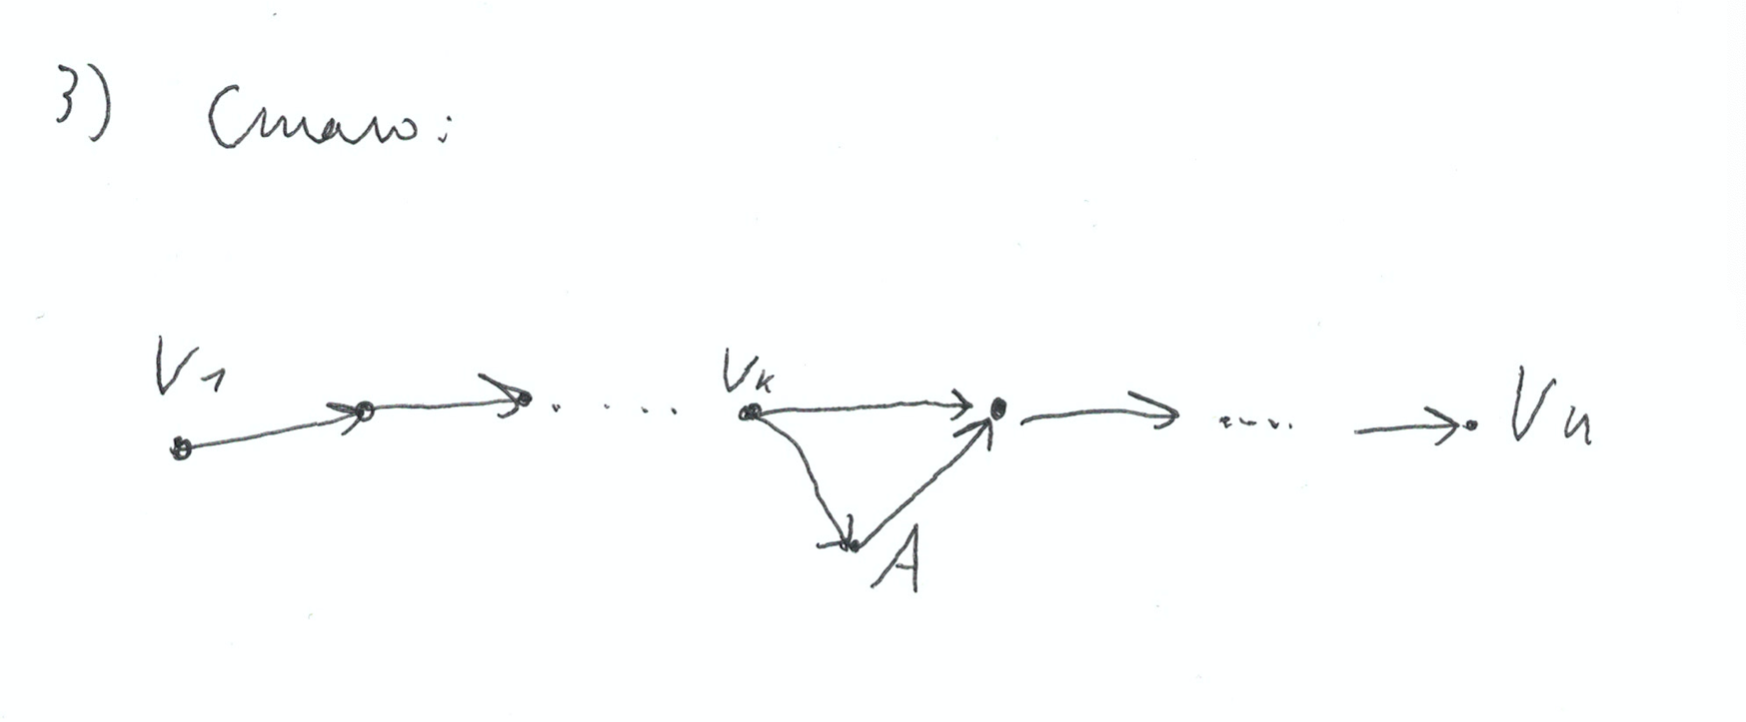
\includegraphics[scale=0.4]{6.3.png}
\end{center}
\begin{center}
\textbf{Верно}
\end{center}
\end{enumerate}
$\rightarrow$ доказано по индукции.

\section*{Номер 7 }
Возьмем граф G на n вершинах из 6го номера.Тогда поменяем в нем ориентацию одного любого ребра и рассмотрим полученный граф, назовем его $G'$. По условию 7й задачи меняем в $G'$ ориентацию этого же ребра и вновь возвращаемся к графу G. Но мы знаем, по доказанному в 6м номере, что в этом графе есть простой путь, проходящий через все вершины $\rightarrow$ он сильно связан.
\begin{center}
\textbf{Ч.Т.Д}
\end{center}
\end{document}
